\chapter{Realisation}
\label{ch:Realisation}
This chapter describes the realisation of the project, and provides some insights into the ideas, which led to the current implementation. The implementation was written in Python 3.6.9 and Tensorflow 2.1. To standardise the realisation, standard docker images are used which are provided by Tensorflow, called \texttt{tensorflow/tensorflow:2.1.0-py3}, respectively \texttt{tensorflow/tensorflow:2.1.0-gpu-py3} to utilise the GPU.

\section{Project components}
\label{sec:Project-Components}
The project repository, which is shown in figure \ref{fig:Project-Overview-Source}, shows the overall structure of the realisation. All of the source code for the project is located in the \texttt{src} directory, which is further divided into folders for the components of the project. These components are illustrated in figure \ref{sec:Project-Components}. The figure shows that there are two main python scripts which orchestrate the training of the triplet loss and the classifier (\texttt{train-classifier.py} and \texttt{train-triplet-loss.py}). 

\begin{figure}[ht]
    \dirtree{%
    .1 src/.
    .2 feature-extractor/ \ldots{} (audio representations).
    .2 input-pipeline/ \ldots{} (triplet input pipeline).
    .2 loss/ \ldots{} (implementation of loss functions).
    .2 models/ \ldots{} (implementation of models).
    .2 training/ \ldots{} (training utility functions).
    .2 utils/ \ldots{} (contains various utility functions).
    .2 train-classifier.py \ldots{} (training procedure for classifier).
    .2 train-triplet-loss.py \ldots{} (training procedure of triplet loss).
    }
\caption{Project components of the \texttt{src} directory}
\label{fig:Project-Components}
\end{figure}
\noindent
All of the components of the project were designed to be arbitrarily expandable, which is an essential criterion to successfully conduct and validate experiments because with such an architecture the project can be expanded fast and new ideas are implemented rapidly.
\newline
\newline
Each one of these components is described in further detail within this section of the thesis. This includes detailed information about the component as well as their purpose in the whole project.

\subsection{Feature extractor}
\label{sub:Component-Feature-Extractor}
\begin{figure}[htbp]
	\centering
	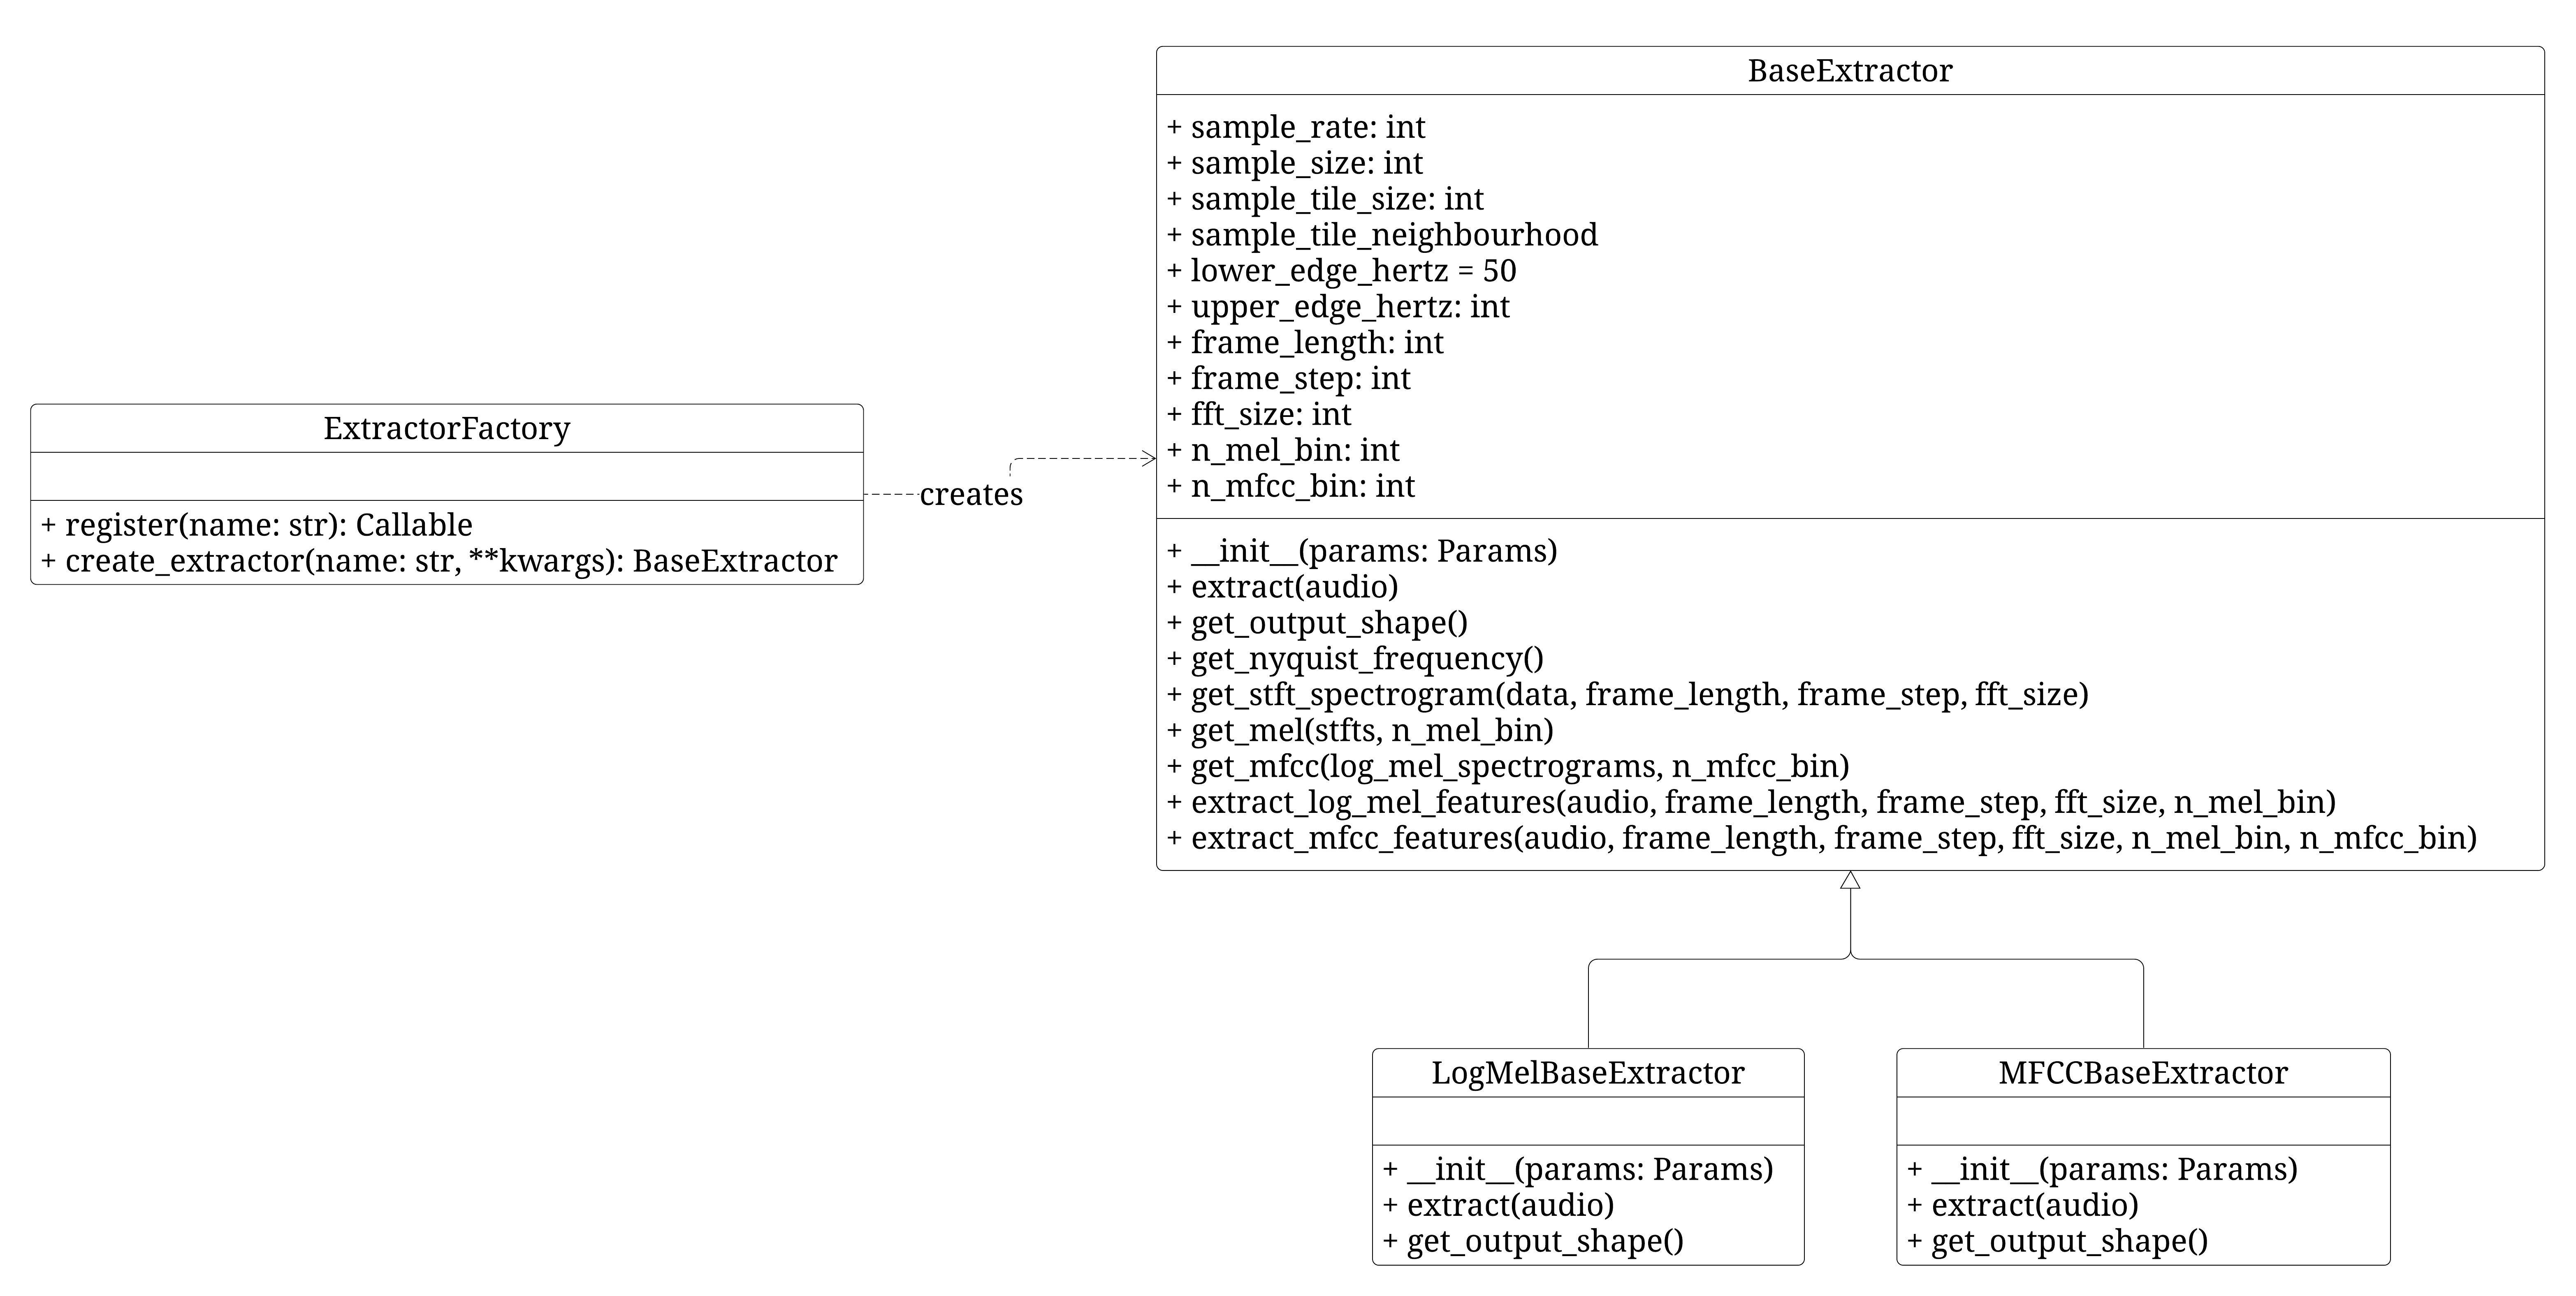
\includegraphics[width=\linewidth]{baa-documentation/img/UML_Feature_Extractor.jpeg}
	\caption{UML diagram of the \flqq feature extractor\frqq}
	\label{fig:UML-Feature-Extractor}
\end{figure}
\noindent
The feature extractor is responsible for representing an audio signal in different feature representations. The structure is shown in figure \ref{fig:UML-Feature-Extractor}, it consists out of a abstract base class (\texttt{BaseExtractor}), two implementations of the base class (\texttt{LogMelBaseExtractor} and \texttt{MFCCBaseExtractor}) and a factory class (\texttt{ExtractorFactory}). The idea is that the abstract \texttt{BaseExtractor} implements the used methods to calculate a feature representation, such as calculating the \gls{STFT}, and the implementations (\texttt{LogMelBaseExtractor} and \texttt{MFCCBaseExtractor}) only have to call the calculations in the correct sequence. The factory class \texttt{ExtractorFactory} instantiates a specified \texttt{BaseExtractor} implementation given the name in the registry. The factory is implemented using the python decorator pattern.
\newline
\newline
The main benefit of the factory pattern is that the representation used to train the model can be changed using the name of the corresponding extractor, where the name can be used as a hyperparameter. Due to using the factory pattern, the class is arbitrarily expandable, since it only needs to implement the abstract \texttt{BaseExtractor} and can then be used as a representation.

\subsection{Input pipeline}
\label{sub:Component-Input-pipeline}

\subsection{Loss}
\label{sub:Component-Loss}

\subsection{Training}
\label{sub:Component-Training}

\subsection{Utils}
\label{sub:Component-Utils}

\section{Data set}
\label{sec:Data-Set}

\subsection{Data set cleaning}
\label{sub:Data-Set-Cleaning}

\subsection{Statistical analysis of the data set}
\label{sub:Statistical-Analysis-Data-Set}

\section{Training}
\label{sec:Training}

\section{Prototype}
\label{sec:Prototype}
